\documentclass{beamer}
\usepackage[utf8]{inputenc}
\usepackage{graphicx, epsfig}
\usepackage{amsmath,mathrsfs,amsfonts,amssymb}
%\usepackage{subfig}
\usepackage{floatflt}
\usepackage{epic,ecltree}
\usepackage{mathtext}
\usepackage{fancybox}
\usepackage{fancyhdr}
\usepackage{multirow}
\usepackage{enumerate}
\usepackage{epstopdf}
\usepackage{multicol}
\usepackage{algorithm}
\usepackage[noend]{algorithmic}
\def\algorithmicrequire{\textbf{Input:}}
\def\algorithmicensure{\textbf{Output:}}
\usetheme{default}%{Singapore}%{Warsaw}%{Warsaw}%{Darmstadt}
\usecolortheme{default}
\setbeamerfont{title}{size=\Huge}
\setbeamertemplate{footline}[page number]{}
\setbeamerfont{title}{size=\Huge}
\beamertemplatenavigationsymbolsempty

% latin bold lower
\newcommand{\ba}{\mathbf{a}} 
\newcommand{\bc}{\mathbf{c}} 
\newcommand{\be}{\mathbf{e}} 
\newcommand{\bh}{\mathbf{h}} 
\newcommand{\bp}{\mathbf{p}} 
\newcommand{\bt}{\mathbf{t}} 
\newcommand{\bu}{\mathbf{u}} 
\newcommand{\bv}{\mathbf{v}} 
\newcommand{\bw}{\mathbf{w}} 
\newcommand{\bx}{\mathbf{x}} 
\newcommand{\by}{\mathbf{y}} 
\newcommand{\bz}{\mathbf{z}} 

% latin bold upper
\newcommand{\bA}{\mathbf{A}} 
\newcommand{\bC}{\mathbf{C}} 
\newcommand{\bI}{\mathbf{I}} 
\newcommand{\bM}{\mathbf{M}} 
\newcommand{\bT}{\mathbf{T}} 
\newcommand{\bU}{\mathbf{U}} 
\newcommand{\bW}{\mathbf{W}} 
\newcommand{\bX}{\mathbf{X}} 
\newcommand{\bY}{\mathbf{Y}} 
\newcommand{\bZ}{\mathbf{Z}} 

% latin cal upper
\newcommand{\cL}{\mathcal{L}} 
\newcommand{\cN}{\mathcal{N}} 
\newcommand{\cS}{\mathcal{S}} 
\newcommand{\cT}{\mathcal{T}} 
\newcommand{\cW}{\mathcal{W}} 
\newcommand{\cX}{\mathcal{X}} 
\newcommand{\cZ}{\mathcal{Z}} 

% latin cal upper
\newcommand{\bbE}{\mathbb{E}} 
\newcommand{\bbP}{\mathbb{P}} 
\newcommand{\bbR}{\mathbb{R}} 

% greek bold lower
\newcommand{\bepsilon}{\boldsymbol{\epsilon}} 
\newcommand{\btheta}{\boldsymbol{\theta}} 
\newcommand{\blambda}{\boldsymbol{\lambda}} 
\newcommand{\bmu}{\boldsymbol{\mu}} 
\newcommand{\bsigma}{\boldsymbol{\sigma}} 
\newcommand{\bphi}{\boldsymbol{\phi}} 

% greek bold upper
\newcommand{\bSigma}{\boldsymbol{\Sigma}} 

\DeclareMathOperator*{\argmin}{arg\,min}
\DeclareMathOperator*{\argmax}{arg\,max}

\newcommand{\createdgmtitle}[1]{\title[\hbox to 56mm{Deep Generative Models  \hfill\insertframenumber\,/\,\inserttotalframenumber}]
	{\vspace{1cm} \\ Deep Generative Models \\ Lecture #1 \\ \vspace{-0.5cm}}
	\author{Roman Isachenko \\ \vspace{-0.5cm}}
	\institute{
\includegraphics[width=3cm]{../utils/ozonmasterslogo}
	\\Ozon Masters
	}
	\date{Spring, 2021}
}

\newcommand\myfootnote[1]{%
  \tikz[remember picture,overlay]
  \draw (current page.south west) +(1in + \oddsidemargin,0.5em)
  node[anchor=south west,inner sep=0pt]{\parbox{\textwidth}{%
      \rlap{\rule{10em}{0.4pt}}\raggedright\scriptsize#1}};}

\newcommand\myfootnotewithlink[2]{%
  \tikz[remember picture,overlay]
  \draw (current page.south west) +(1in + \oddsidemargin,0.5em)
  node[anchor=south west,inner sep=0pt]{\parbox{\textwidth}{%
      \rlap{\rule{10em}{0.4pt}}\raggedright\scriptsize\href{#1}{\textit{#2}}}};}
\createdgmtitle{2}
%--------------------------------------------------------------------------------
\begin{document}
%--------------------------------------------------------------------------------
\begin{frame}
%\thispagestyle{empty}
\titlepage
\end{frame}
%=======
\begin{frame}{Generative models zoo}
    \begin{figure}
        \centering
        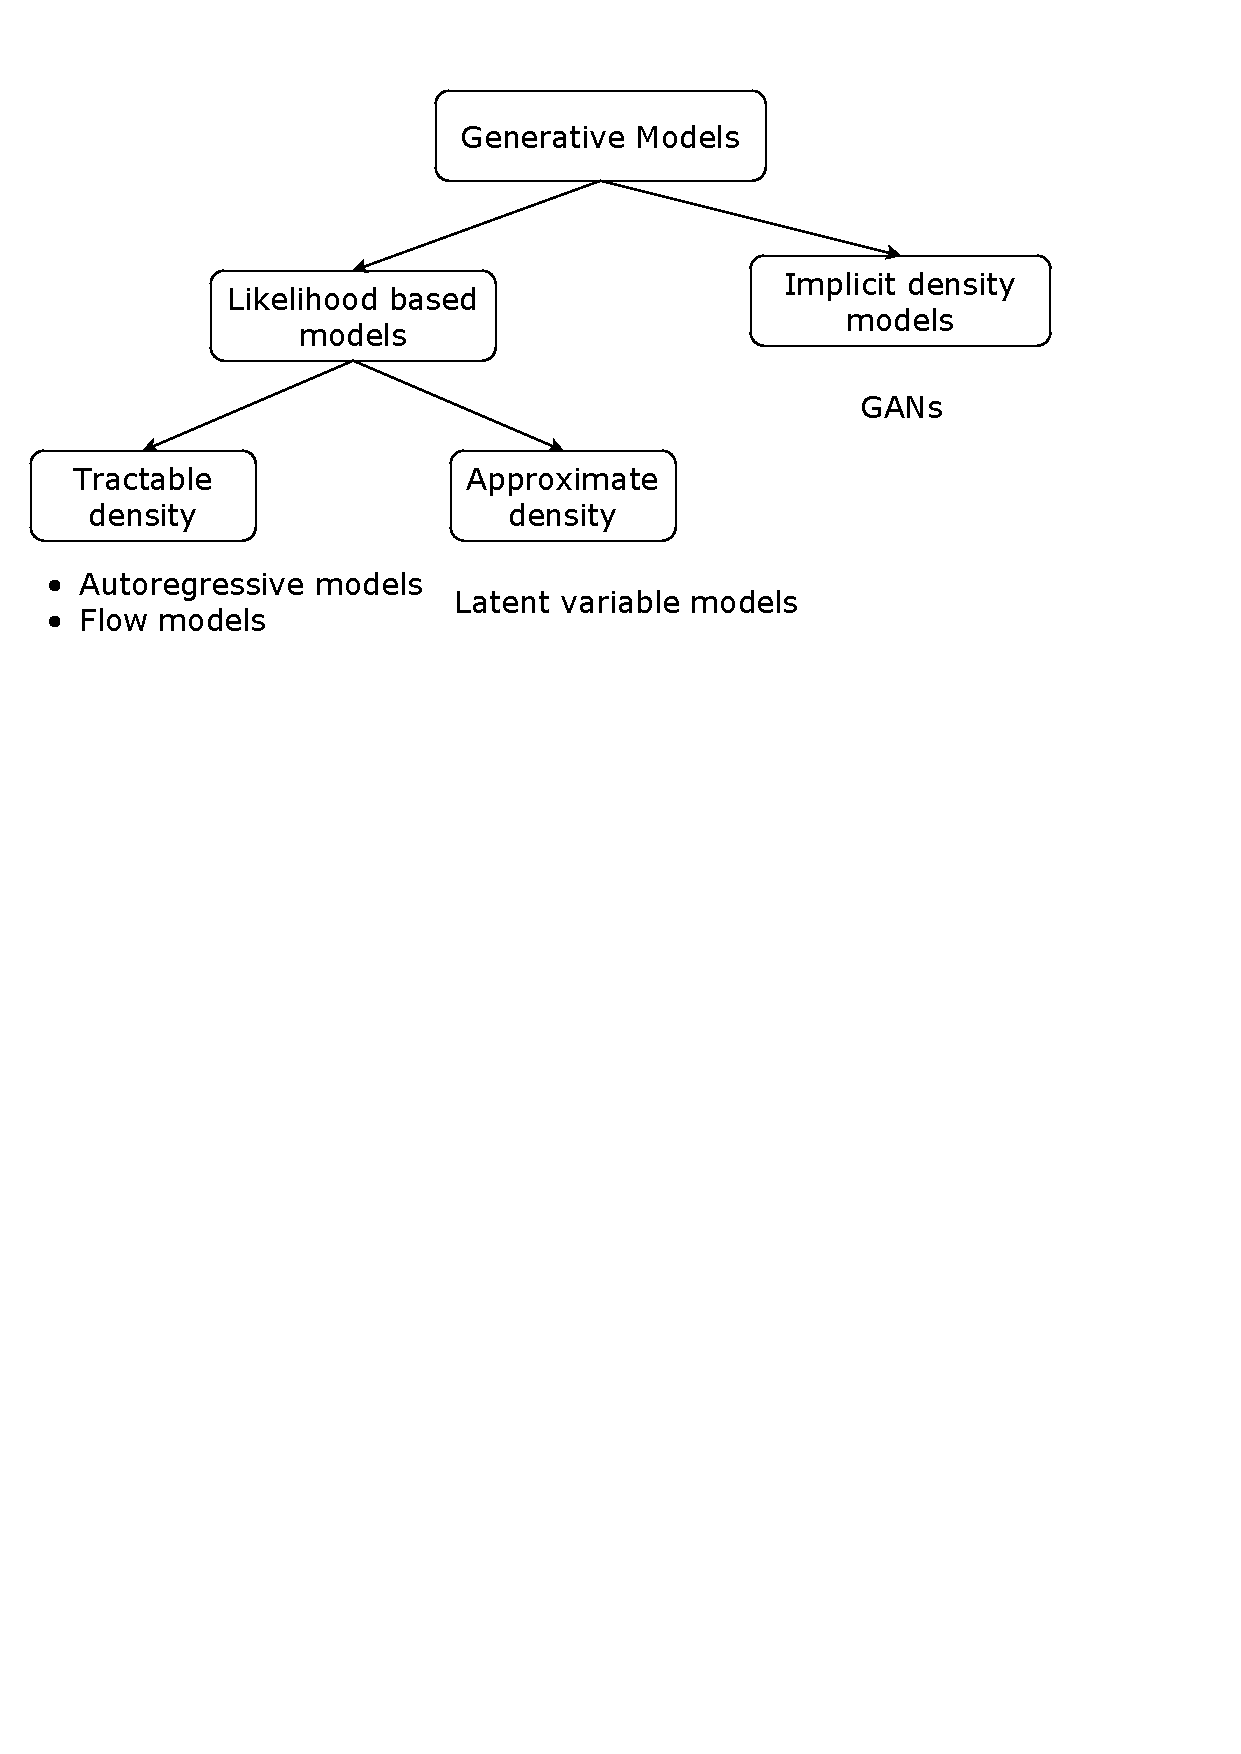
\includegraphics[width=1.0\linewidth]{figs/generative_models_zoo.pdf}
        \label{fig:generative_models_zoo}
    \end{figure}
\end{frame}
%=======
\begin{frame}{Bayesian framework}
\begin{itemize}
    \item $\bx$ -- samples;
    \item $\by$ -- target variables;
    \item $\btheta$ -- model parameters.
\end{itemize}
\begin{minipage}[t]{0.5\columnwidth}
\begin{block}{Discriminative}
    \[
        p(\by, \btheta | \bx) = p(\by | \bx, \btheta) p(\btheta)
    \]
    \begin{itemize}
        \item Find conditional probability of $\by$ given $\bx$. \\
        \item Samples $\bx$ are given. \\
        \item Used for classification, regression.
    \end{itemize}
\end{block}
\end{minipage}%
\begin{minipage}[t]{0.5\columnwidth}
\begin{block}{Generative}
    \[
        p(\by, \bx, \btheta) = p(\by, \bx | \btheta) p(\btheta)
    \]
    \begin{itemize}
        \item Find joint probability of $(\bx, \by)$.
        \item Samples $\bx$ should be modelled. \\
        \item Generation of new samples $(\bx, \by)$.
    \end{itemize}
\end{block}
\end{minipage}
\end{frame}
%=======
\begin{frame}{Generative models}
    We age given samples $\{\bx_i\}_{i=1}^n \in X$ from unknown distribution $p(\bx)$.
    
    \begin{block}{Goal}
    	We would like to learn a distribution $p(\bx)$ for 
    	\begin{itemize}
    	    \item evaluating $p(\bx)$ for new samples;
    	    \item sampling from $p(\bx)$.
    	\end{itemize}
    \end{block}
    \begin{block}{Challenge}
    	 Data is complex and high-dimensional (curse of dimensionality).
    \end{block}
    \begin{block}{Solution}
        Fix probabilistic model $p(\bx | \btheta)$~-- the set of parameterized distributions . \\
        Instead of searching true $p(\bx)$ over all probability distributions, learn function approximation $p(\bx | \btheta) \approx p(\bx)$.
    \end{block}
\end{frame}
%=======
\begin{frame}{Latent variable models (LVM)}
    Suppose that our probabilistic model is $p(\bx, \bz | \btheta)$ instead of $p(\bx | \btheta)$.
    \begin{itemize}
        \item Here $\bz$ are latent variables.
        \item We observe only samples $\bx$. 
        \item Latent variables $\bz$ are unknown.
        \item Parameters $\btheta$ are not random.
    \end{itemize}
    \begin{block}{MLE problem for LVM}
    \vspace{-0.3cm}
    \begin{multline*}
        \btheta^* = \argmax_{\btheta} p(\bX, \bZ | \btheta) = \argmax_{\btheta} \prod_{i=1}^n p(\bx_i, \bz_i | \btheta) = \\ = \argmax_{\btheta} \sum_{i=1}^n \log p(\bx_i, \bz_i | \btheta).
    \end{multline*}
    \vspace{-0.1cm}
    \end{block}
    What if $\btheta$ are random variables with distribution $p(\btheta)$?
\end{frame}
%=======
\begin{frame}{Bayesian framework}
    What if $\btheta$ are random variables with distribution $p(\btheta)$? \\
    Before we get any data, we do not know anything about $\btheta$ except the \textbf{prior}  distribution $p(\btheta)$. \\
    When we get data, we could change the \textbf{prior} distribution to the \textbf{posterior}. 
    \begin{block}{Bayes theorem}
    \[
        p(\btheta | \bX, \bZ) = \frac{p(\bX, \bZ | \btheta) p(\btheta)}{p(\bX, \bZ)} = \frac{p(\bX, \bZ | \btheta) p(\btheta)}{\int p(\bX , \bZ | \btheta) p(\btheta) d \btheta} 
    \]
    \end{block}
    \begin{block}{Full Bayesian inference}
    \[
        p(\bx^* | \bX, \bZ) = \int p(\bx^* | \btheta) p(\btheta | \bX, \bZ) d \btheta
    \]
    \end{block}
\end{frame}
%=======
\begin{frame}{Bayesian framework}
    \begin{block}{Full Bayesian inference}
    \[
        p(\bx^* | \bX, \bZ) = \int p(\bx^* | \btheta) p(\btheta | \bX, \bZ) d \btheta
    \]
    \end{block}
    \begin{block}{Maximum a posteriori (MAP)}
    \vspace{-0.2cm}
    \[
        \btheta^* = \argmax_{\btheta} p(\btheta | \bX, \bZ) = \argmax_{\btheta} \bigl(\log p(\bX, \bZ | \btheta) + \log p(\btheta) \bigr)
    \]
    \vspace{-0.2cm}
    \[
    p(\bx^* | \bX, \bZ) = \int p(\bx^* | \btheta) p(\btheta | \bX, \bZ) d \btheta \approx p(\bx^* | \btheta^*).
    \]
    \end{block}
\end{frame}
%=======
\begin{frame}{Latent variable models}
    \begin{block}{MLE problem}
    \vspace{-0.3cm}
    \[
        \btheta^* = \argmax_{\btheta} p(\bX | \btheta) = \argmax_{\btheta} \prod_{i=1}^n p(\bx_i | \btheta) = \argmax_{\btheta} \sum_{i=1}^n \log p(\bx_i | \btheta).
    \]
    \vspace{-0.3cm}
    \end{block}
    \begin{block}{Challenge}
    $p(\bx | \btheta)$ could be intractable.
    \end{block}
    \begin{block}{Extend probabilistic model}
    Introduce latent variable $\bz$ for each sample $\bx$
    \[
        p(\bx, \bz | \btheta) = p(\bx | \bz, \btheta) p(\bz); \quad 
        \log p(\bx, \bz | \btheta) = \log p(\bx | \bz, \btheta) + \log p(\bz).
    \]
    \[
        p(\bx | \btheta) = \int p(\bx, \bz | \btheta) d\bz = \int p(\bx | \bz, \btheta) p(\bz) d\bz.
    \]
    \end{block}
\end{frame}
%=======
\begin{frame}{Latent variable models}
    \[
    \log p(\bx | \btheta) = \log \int p(\bx | \bz, \btheta) p(\bz) d\bz \rightarrow \max_{\btheta}
    \]
    \vspace{-0.6cm}
    \begin{block}{Examples}
    \begin{minipage}[t]{0.45\columnwidth}
		\textit{Mixture of gaussians} \\
		\vspace{-0.5cm}
		\begin{figure}
			\centering
			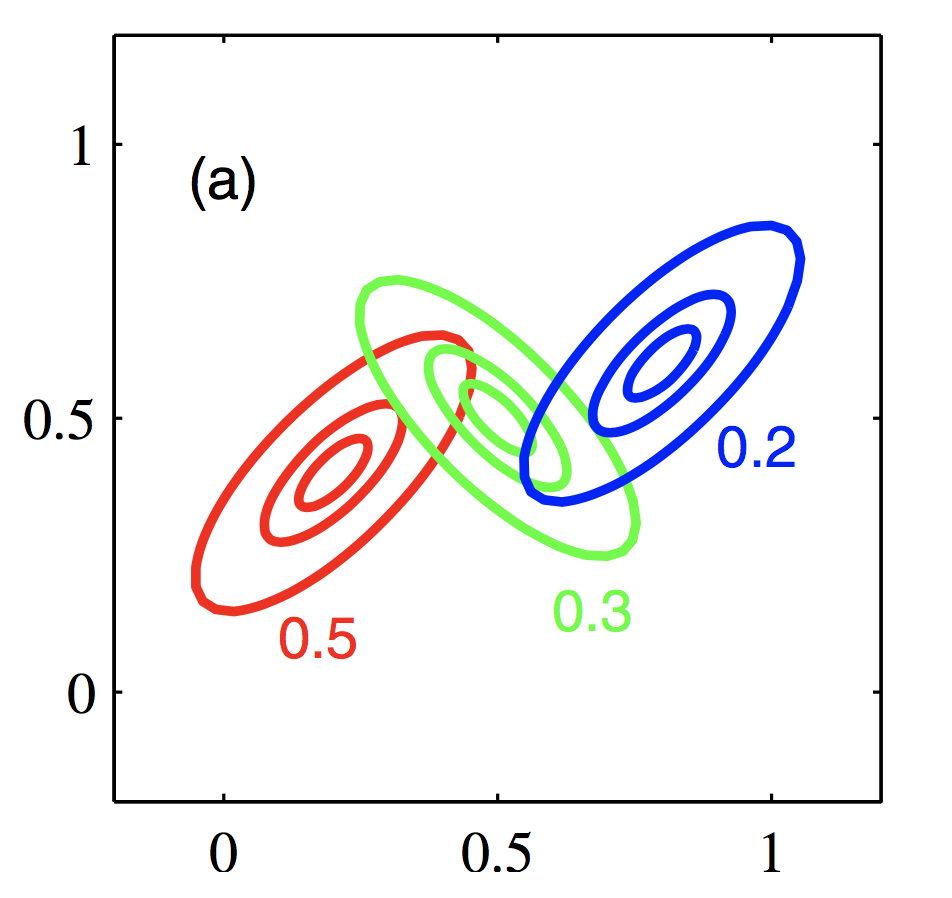
\includegraphics[width=0.75\linewidth]{figs/mixture_of_gaussians.png}
		\end{figure}
		\vspace{-0.5cm}
	    \begin{itemize}
	        \item $p(\bx | \bz, \btheta) = \mathcal{N}(\bx | \boldsymbol{\mu}_\bz, \boldsymbol{\Sigma}_\bz)$
	        \item $p(\bz) = \text{Cat}(\bz | \boldsymbol{\pi})$
	    \end{itemize}
	\end{minipage}%
	\begin{minipage}[t]{0.53\columnwidth}
		\textit{PCA model} \\
		\vspace{-0.5cm}
		\begin{figure}
			\centering
			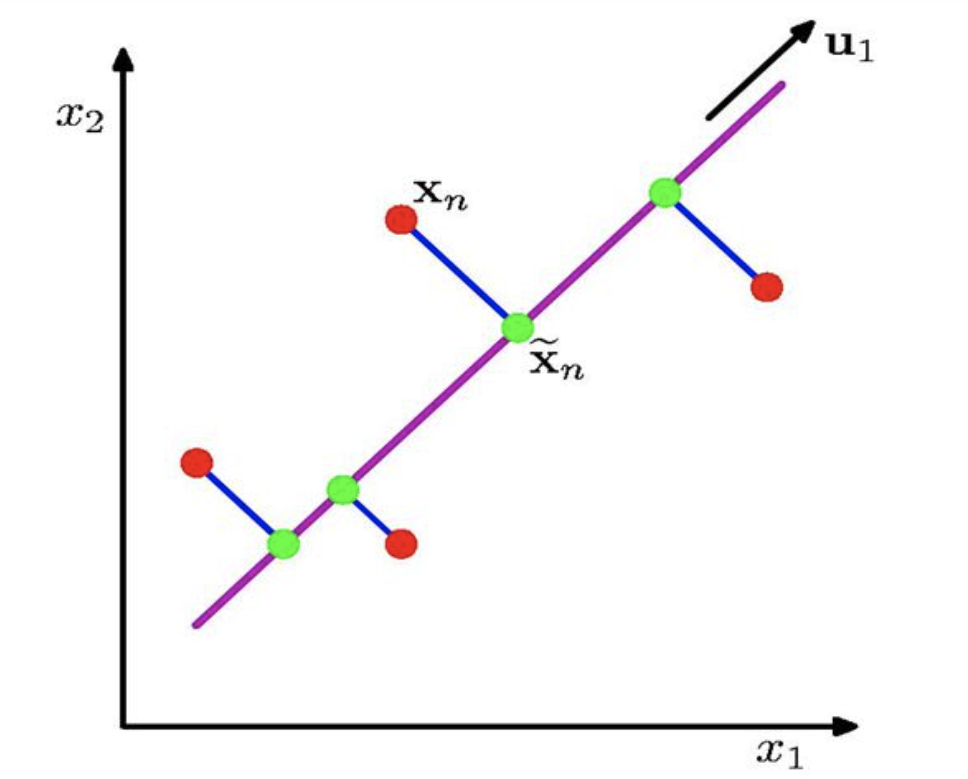
\includegraphics[width=.7\linewidth]{figs/pca.png}
		\end{figure}
		\vspace{-0.5cm}
		\begin{itemize}
	        \item $p(\bx | \bz, \btheta) = \mathcal{N}(\bx | \mathbf{W} \bz + \boldsymbol{\mu}, \boldsymbol{\Sigma}_\bz)$
	        \item $p(\bz) = \mathcal{N}(\bz | 0, \mathbf{I})$
	    \end{itemize}
	\end{minipage}
	\end{block}
\myfootnote{Bishop\,C. Pattern Recognition and Machine Learning, 2006}
\end{frame}
%=======
\begin{frame}{Latent variable models}
    \[
    \log p(\bx | \btheta) = \log \int p(\bx | \bz, \btheta) p(\bz) d\bz \rightarrow \max_{\btheta}
    \]
	\textbf{PCA goal:} Project original data $\bX$ onto low latent space while maximizing the variance of the projected data. 
	\begin{figure}
		\centering
		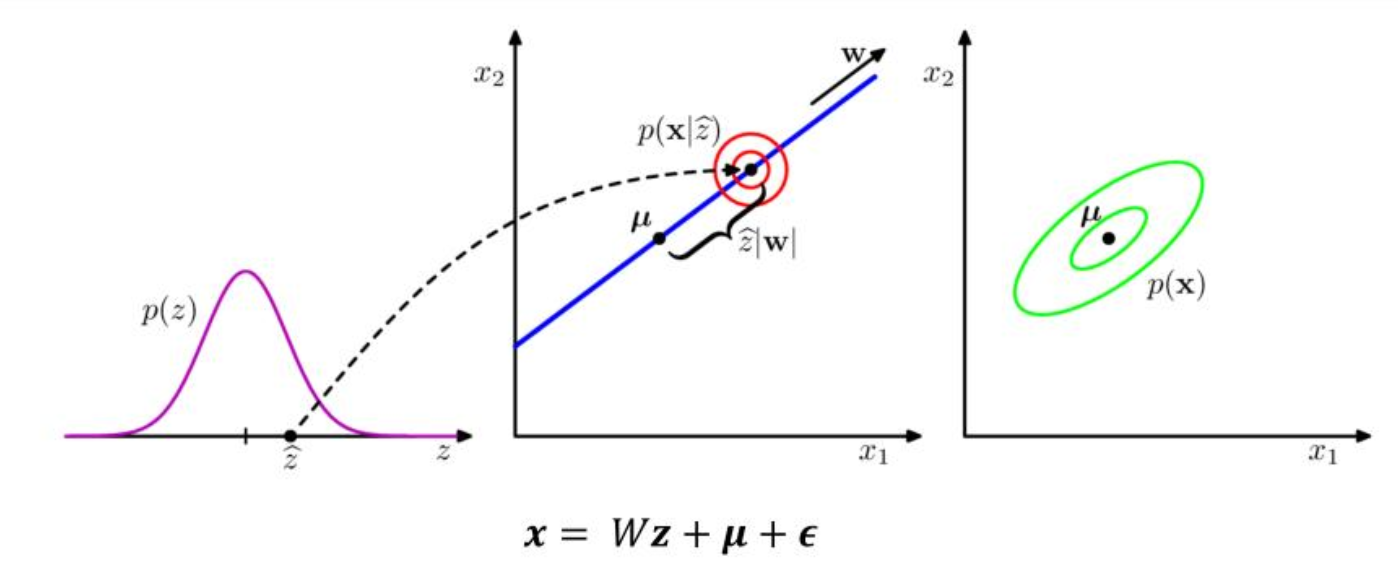
\includegraphics[width=.7\linewidth]{figs/bayesian_pca.png}
	\end{figure}
	\vspace{-0.5cm}
	\begin{itemize}
        \item $p(\bx | \bz, \btheta) = \mathcal{N}(\bx | \mathbf{W} \bz + \boldsymbol{\mu}, \boldsymbol{\Sigma}_\bz)$
        \item $p(\bz) = \mathcal{N}(\bz | 0, \mathbf{I})$
    \end{itemize}
    
    \myfootnote{Bishop\,C. Pattern Recognition and Machine Learning, 2006}
    
\end{frame}
%=======
\begin{frame}{Incomplete likelihood}
        \begin{block}{MLE problem}
            \vspace{-0.3cm}
            \begin{multline*}
                \vspace{-0.3cm}
                \btheta^* = \argmax_{\btheta} p(\bX, \bZ | \btheta) = \argmax_{\btheta} \prod_{i=1}^n p(\bx_i, \bz_i | \btheta) = \\ = \argmax_{\btheta} \sum_{i=1}^n \log p(\bx_i, \bz_i | \btheta).
            \end{multline*}
            \vspace{-0.3cm}
        \end{block}
	Since $\bZ$ is unknown, maximize \textbf{incomplete likelihood}.
    \begin{block}{MILE problem}
        \vspace{-0.3cm}
    	\begin{multline*}
        	\btheta^* = \argmax_{\btheta} \log p(\bX| \btheta) = \argmax_{\btheta} \log \int p(\bX, \bZ | \btheta) d \bZ = \\ = \argmax_{\btheta} \log \int p(\bX| \bZ, \btheta) p(\bZ) d\bZ.
    	\end{multline*}
        \vspace{-0.3cm}
	\end{block}
	
\end{frame}
%=======
\begin{frame}{Variational lower bound}
	\begin{multline*}
		\log p(\bX| \btheta) 
		= \log \frac{p(\bX, \bZ| \btheta)}{p(\bZ|\bX, \btheta)} = \\ 
		= \int q(\bZ) \log \frac{p(\bX, \bZ| \btheta)}{p(\bZ|\bX, \btheta)}d\bZ
		= \int q(\bZ) \log \frac{p(\bX, \bZ| \btheta) q(\bZ)}{p(\bZ|\bX, \btheta) q(\bZ)} d\bZ = \\
		= \int q(\bZ) \log \frac{p(\bX, \bZ | \btheta)}{q(\bZ)}d\bZ + \int q(\bZ) \log \frac{q(\bZ)}{p(\bZ|\bX, \btheta)}d\bZ = \\ 
		= \mathcal{L} (q, \btheta) + KL(q(\bZ) || p(\bZ|\bX, \btheta)) \geq \mathcal{L} (q, \btheta).
	\end{multline*}
	\begin{block}{Kullback-Leibler divergence}
	    \begin{itemize}
	        \item $KL(q || p) \geq 0$;
	        \item $KL(q || p) = 0 \Leftrightarrow q \equiv p$.
	    \end{itemize}
	\end{block}
\end{frame}
%=======
\begin{frame}{Variational lower bound}
\[
    \log p(\bX| \btheta) = \mathcal{L} (q, \btheta) + KL(q(\bZ) || p(\bZ|\bX, \btheta)) \geq \mathcal{L} (q, \btheta).
\]
\begin{block}{Evidence Lower Bound (ELBO)}
\begin{align*}
    \mathcal{L} (q, \btheta) &= \int q(\bZ) \log \frac{p(\bX, \bZ | \btheta)}{q(\bZ)}d\bZ = \\ 
    &= \int q(\bZ) \log p(\bX | \bZ, \btheta) d\bZ + \int q(\bZ) \log \frac{p(\bZ)}{q(\bZ)}d\bZ \\ 
    &= \mathbb{E}_{q} \log p(\bX | \bZ, \btheta) - KL (q(\bZ) || p(\bZ))
\end{align*}
\end{block}
Instead of maximizing incomplete likelihood, maximize ELBO
\[
    \max_{\theta} p(\bX | \btheta) \quad \rightarrow \quad \max_{q, \theta} \mathcal{L} (q, \btheta).
\]
    
\end{frame}
%=======
\begin{frame}{EM-algorithm}
	\[
		\mathcal{L} (q, \btheta)  = \int q(\bZ) \log p(\bX | \bZ, \btheta) d\bZ + \int q(\bZ) \log \frac{p(\bZ)}{q(\bZ)}d\bZ.
	\]
	\begin{block}{Block-coordinate optimization}
	\begin{itemize}
		\item Initialize $\btheta^*$;
		\item E-step
		\[
			q(\bZ) = \argmax_q \mathcal{L} (q, \btheta^*) = \argmin_q KL(q || p) =
			 p(\bZ| \bX, \btheta^*);
		\]
		\item M-step
		\[
			\btheta^* = \argmax_{\btheta} \mathcal{L} (q, \btheta);
		\]
		\item Repeat E-step and M-step until convergence.
	\end{itemize}
	\end{block}
\end{frame}
%=======
\begin{frame}{Amortized variational inference}
    \begin{block}{E-step}
    \vspace{-0.3cm}
    \[
		q(\bZ) = \argmax_q \mathcal{L} (q, \btheta^*) = \argmin_q KL(q || p) =
		 p(\bZ| \bX, \btheta^*).
	\]
	could be \textbf{intractable}.
    \end{block}
	\begin{block}{Idea}
	Restrict a family of all possible distributions $q(\bz)$ to a particular parametric class conditioned on sample: $q(\bz|\bx, \bphi)$.
	\end{block}
	
	\textbf{Variational Bayes}
	\begin{itemize}
		\item E-step
		\[
		\bphi_k = \bphi_{k-1} + \left.\eta \nabla_{\bphi} \mathcal{L}(\bphi, \btheta_{k-1})\right|_{\bphi=\bphi_{k-1}}
		\]
		\item M-step
		\[
		\btheta_k = \btheta_{k-1} + \left.\eta \nabla_{\btheta} \mathcal{L}(\bphi_k, \btheta)\right|_{\btheta=\btheta_{k-1}}
		\]
	\end{itemize}
\end{frame}
%=======
\begin{frame}{Summary}
\end{frame}
\end{document} 